\chapter{Derivatives}

In calculus, the derivative of a function represents the rate at which
the function is changing at a particular point. It is a fundamental
concept that has vast applications in various fields, including
physics.\index{derivative}

\section{Definition}

The derivative of a function $f(x)$ at a point $x$ is defined as the limit:

\begin{equation}
f'(x) = \lim_{{h \to 0}} \frac{f(x+h) - f(x)}{h}
\end{equation}

provided this limit exists. In words, the derivative of $f$ at $x$ is
the limit of the rate of change of $f$ at $x$ as the change in $x$
approaches zero.

\section{Applications in Mathematics}
\subsection{l'Hospital's Rule}
Consider the function $h(x) = \frac{\ln{x}}{x-1}$ and suppose we are interested in the behavior of $h(x)$ around $x=1$. If we apply the Quotient Rule, we get an indeterminate result: $$\lim_{x \to 1}\frac{\ln{x}}{x-1} = \frac{0}{0}$$ Looking at the graph of $h(x)$, we can guess that $\lim_{x \to 1}\frac{\ln{x}}{x-1} = 1$. 

\begin{tikzpicture}
\begin{axis}
    [clip=true,
    xmin=0, xmax=4,
    ymin=0, ymax=4,
    axis lines=left
    ]
    \addplot[blue, domain=0.01:4, samples=100]{ln(x)/(x-1)};
    \addplot[samples=50, black, dashed] coordinates{(1, 0)(1,1)};
    \addplot[samples=50, black, dashed] coordinates{(0, 1)(1,1)};
    \addplot[mark=*, fill=white, draw=blue] coordinates{(1, 1)};
\end{axis}
\end{tikzpicture}

Let's examine the numerator and denominator separately: we'll define $f(x)=\ln{x}$ and $g(x) = x-1$. 

\begin{tikzpicture}
    \begin{axis}
    [clip=false,
    xmin=0, xmax=3,
    ymin=-1, ymax=2,
    axis lines = center]
    \addplot[blue, samples=100, domain=1/e:3]{ln(x)}
    node[right, pos=1]{$f(x)$};
    \addplot[red, samples=100, domain=0:3]{x-1}
    node[right, pos=1]{$g(x)$};
    \end{axis}
\end{tikzpicture}

If we zoom in very far around $x=1$, the graphs begin to look linear:

\begin{tikzpicture}
    \begin{axis}
    [clip=false,
    xmin=0.9, xmax=1.1,
    ymin=-0.1, ymax=0.1,
    axis lines = center]
    \addplot[blue, samples=100, domain=0.9:1.1]{ln(x)}
    node[right, pos=0.9]{$f(x)$};
    \addplot[red, samples=100, domain=0.9:1.1]{x-1}
    node[right, pos=1]{$g(x)$};
    \end{axis}
\end{tikzpicture}

We can approximate these graphs as linear functions with slopes $m_1$ and $m_2$, so that the blue curve is approximated as $y=m_1(x-1)$ and the red curve is approximated as $y=m_2(x-1)$. The ratio of the functions would then be $$\frac{m_1(x-1)}{m_2(x-1)}=\frac{m_1}{m_2}$$ which is the same as the ratio of the derivatives of our linear approximations. This suggests l'Hospital's rule, that the limit of a ratio is the same as the limit of the ratio of the derivatives for certain indeterminate forms: $$\lim_{x\to a}\frac{f(x)}{g(x}=\lim_{x\to a}\frac{f'(x)}{g'(x)}$$.

Let's apply l'Hospital's rule to our limit of $h(x)$:
$$\lim_{x\to 1}\frac{\ln{x}}{x-1}=\lim_{x \to 1}\frac{\frac{d}{dx}\ln{x}}{\frac{d}{dx}(x-1)}=\lim_{x \to 1}\frac{\frac{1}{x}}{1}=1$$

Notice our result with l'Hospital's rule matches our guess based on the graph of $h(x) = \frac{\ln{x}}{x-1}$. 

L'Hospital's rule also applies to the indeterminate result $\frac{\pm \infty}{\pm \infty}$. For a limit of the form $\lim_{x\to a}\frac{f(x)}{g(x)}$, l'Hospital's rule applies if:
\begin{enumerate}
    \item the original limit is of the indeterminate form $\frac{0}{0}$ or $\frac{\pm \infty}{\pm \infty}$
    \item $f$ and $g$ are differentiable on an interval containing $a$ (but possibly not differentiable at $a$)
    \item $g'(x) \neq 0$ on said interval
\end{enumerate}



\subsection{Mean Value Theorem}

The Mean Value Theorem (MVT) states that on an interval $[a, b]$ where a continuous function $f$ is differentiable on an open interval $(a, b)$, there is at least one point where the tangent line to $f$ has the same slope as a line connecting the points $(a, f(a))$ and $(b, f(b))$. Consider the graph of $f(x) = x^2$ below. The line connecting the points $(-1, 1)$ and $(2, 4)$ has a slope of $\frac{1}{2}$. MVT tells us there must be \textit{at least one} point, $c$, on the interval $x \in (-1, 2)$ where $f'(c) = \frac{1}{2}$. We can find this point by setting $f'(x)$ equal to $\frac{1}{2}$: $$2x=\frac{1}{2} \rightarrow x=\frac{1}{4}$$

Examining the graph, you can see that the tangent at $f(\frac{1}{4})$ (the black line) is parallel to the line connecting $(-1, f(-1))$ and $(2, f(2))$. 

\begin{tikzpicture}
    \begin{axis}
        [ymin=-2, xmin=-2, xmax=2, axis lines = left]
        \addplot[blue, samples=50]{x^2};
        \addplot[red, mark=*]coordinates {(-1, 1)};
        \addplot[red, mark=*] coordinates {(2, 4)};
        \addplot[domain=-2:2, red] coordinates{(-1, 1)(2, 4)};
        \addplot[black, mark=*] coordinates{(0.5, 0.25)};
        \addplot[black, domain=-2:2, samples=50
        ]{x-0.25};
    \end{axis}
\end{tikzpicture}

Note that MVT doesn't tell us \textit{where} $f'(x)$ is parallel to the line connecting $(a, f(a))$ and $(b, f(b))$, just that some value $c$ exists that satisfies the condition. 

Consider a hammer thrown upwards at 5 $\frac{m}{s^2}$ on Earth (where the acceleration due to gravity is approximately $-9.8 \frac{m}{s^2}$). We can use MVT to show that there must be some point in the hammer's path upwards where the velocity of the hammer is exactly equal to its average velocity as it flies through the air. 
The hammer's rise can be described with the function $y(t) = 5t-4.9t^2$. The hammer reaches its peak at approximately $t=0.51$. So, we are looking for some value, $c$, such that $$y'(c) = \frac{y(0.51)-y(0)}{0.51-0}=\frac{5(0.51)-4.9(0.51^2)}{0.51}=\frac{1.2755}{0.51}=2.5$$

Solving $y'(t) = 5-9.8t = 2.5$, we find that the $c$ that satisfies MVT is approximately $0.255$. This result is illustrated on the graph below:

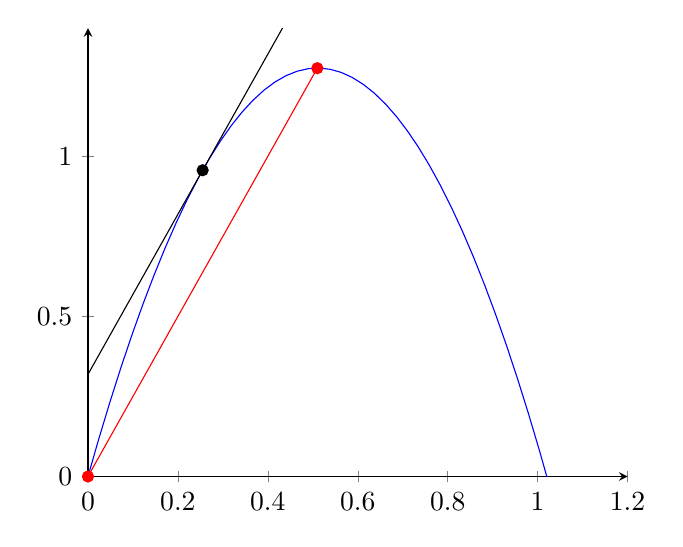
\begin{tikzpicture}
    \begin{axis}[ymin=0,ymax=1.4, xmin=0, xmax=1.2, axis lines=left]
    \addplot[blue, samples=50, domain=0:1.2]{5*x-4.9*x^2};
    \addplot[mark=*, red] coordinates{(0,0)};
    \addplot[mark=*, red] coordinates{(0.51, 1.275)};
    \addplot[red, samples=50]coordinates{(0,0) (0.51, 1.275)};
    \addplot[black, samples=50]{2.5*(x-0.255)+0.9564};
    \addplot[mark=*, black]coordinates{(0.255, 0.9564)};
    \end{axis}
\end{tikzpicture}

\subsubsection{MVT Practice}
\begin{Exercise}
[label=MVT1]
AT 3:30 PM, a car's speedometer reads $30 \frac{mi}{hr}$. At 3:40 PM, it reads $50\frac{mi}{hr}$. Show that at some time between 3:30 and 3:340 PM, the car's acceleration is exactly $120 \frac{mi}{hr^2}$. 
\end{Exercise}
\begin{Answer}
[ref=MVT1]
The speed of a car must a continuous, differentiable function, since your car can't "jump" from one speed to another: it must smoothly accelerate from one speed to another. Therefore, the Mean Value Theorem applies. The average acceleration from 3:30 PM to 3:40 PM is given by:
$$\frac{\text{change in speed}}{\text{change in time}} = \frac{50 \frac{mi}{hr}-30\frac{mi}{hr}}{3:40PM-3:30PM}$$ 
Simplifying and converting minutes to hours, we see the average acceleration is:
$$\frac{20\frac{mi}{hr}}{\frac{1}{6}hr} = 120\frac{mi}{hr^2}$$

Therefore, by MVT, there must be some time between 3:30 and 3:40 PM where the car's acceleration is exactly $120 \frac{mi}{hr^2}$. 
\end{Answer}

\begin{Exercise}
[label=MVT2]
Find the number $c$ that satisfies the MVT on the given interval. 

(a) $f(x) = \sqrt{x}$, $[0, 4]$

(b)$f(x) = e^{-x}$, $[0,2]$

(c)$f(x) = \ln{x}$, $[1,4]$	
\end{Exercise}

\begin{Answer}
[ref=MVT2]
(a) For the domain given, $f(x)$ is defined and differentiable. Finding the slope of the secant line connecting the endpoints:
$$\frac{f(b)-f(a)}{b-a}=\frac{\sqrt{4}-\sqrt{0}}{4-0}=\frac{2}{4}=\frac{1}{2}$$
So we are looking for some number $c$ such that $f'(c) = \frac{1}{2}$. Let's find $f'(x)$:
$$f'(x) = \frac{d}{dx}\sqrt{x}=\frac{1}{2\sqrt{x}}$$
Setting this equal to $\frac{1}{2}$ to find $c$:
$$f'(c) = \frac{1}{2\sqrt{c}}=\frac{1}{2}$$
$$\sqrt{c}=1$$
$$c=1$$

(b)For the domain given, $f(x)$ is defined and differentiable. Finding the slope of the secant line connecting the endpoints:
$$\frac{f(2)-f(0)}{2-0}=\frac{e^{-2}-e^{0}}{2}=\frac{1-e^{2}}{2e^{2}}\approx -0.432$$
And find $f'(x)$:
$$f'(x) = -e^{-x}$$
According to MVT, there must be some $c$ such that $f'(c) \approx-0.432$:
$$-e^{-c} \approx -0.432$$
$$e^{-c}\approx 0.432$$
$$-c \approx \ln{0.432}$$
$$c \approx -\ln{0.432} \approx 0.839$$

(c) For the domain given, $f(x)$ is defined and differentiable. Finding the secant line connecting the endpoints:
$$\frac{f(b)-f(a)}{b-a}=\frac{\ln{4}-\ln{1}}{4-1}=\frac{\ln{4}}{3}\approx 0.462$$
And find $f'(x)$:
$$f'(x) = \frac{1}{x}$$
According to MVT, there must be some $c$ such that $f'(c) \approx 0.462$
$$f'(c) = \frac{1}{c} \approx 0.462$$
$$c \approx \frac{1}{0.462} = 2.164$$
\end{Answer}

\subsection{Using first and second derivatives to describe a function}
\subsubsection{Increasing and Decreasing Intervals}

Let's re-examine our graph showing the height of a hammer tossed in the air:


\begin{tikzpicture}
    \begin{axis}[ymin=0,ymax=1.4, xmin=0, xmax=1.2, axis lines=left]
    \addplot[blue, samples=50, domain=0:1.2]{5*x-4.9*x^2};
    \end{axis}
\end{tikzpicture}

As you can see, the hammer reaches its peak around $t \approx 0.5s$. Let's add tangent lines just before and after the peak of the hammer's path so we can more easily examine how the slope of the graph changes:

\begin{tikzpicture}
    \begin{axis}[ymin=0,ymax=1.4, xmin=0, xmax=1.2, axis lines=left]
    \addplot[blue, samples=50, domain=0:1.2]{5*x-4.9*x^2};
    \addplot[red, samples=50, domain=0.31:0.49]{1.08*x-0.4*1.08+1.216};
    \addplot[red, samples=50, domain=0.11:0.29]{3.04*x-0.2*3.04+0.804};
    \addplot[red, samples=50, domain=0.61:0.79]{-1.86*x+1.86*0.7+1.099};
    \addplot[red, samples=50, domain=0.81:0.99]{-3.82*x+0.9*3.82+0.531};
    \end{axis}
\end{tikzpicture}

As you can see, the slope changes from positive to negative as $t$ increases. That implies that $f'(t)$ also changes from positive to negative. In fact, at the highest point of the hammer's flight, the slope (and therefore $f'(t)$) is exactly zero! In general, 
\begin{enumerate}
\item If $f'(x)>0$ on an interval, then $f(x)$ is increasing on that interval.
\item If $f'(x)<0$ on an interval, then $f(x)$ is decreasing on that interval. 
\end{enumerate}

Example 1: Find where the function $f(x) = 3x^4-4x^3-12x^2+5$ is increasing. 

Solution: We want to find the intervals where $f'(x)>0$. First, we take the derivative to find $f'(x)$:
$$f'(x) = 12x^3-12x^2-24x$$

It will be easier to analyze the value of $f'(x)$ if we factor it so:
$$f'(x) = 12x(x-2)(x+1)$$

To determine where $f'(x)>0$, we start by finding where $f'(x)=0$ (in this case, this is true when $x=-1, 0, 2$). These values of $x$ are called \textit{critical values}, and we will use them to divide $f'(x)$ into intervals. On each of these intervals, $f'(x)$ must be always positive or always negative. This is shown graphically below:

\begin{tikzpicture}
	\begin{axis}[xmin=-2, xmax=3, axis lines=center]
	\addplot[blue, samples=100, domain=-2:3]{12*x*(x-2)*(x+1)};
	\addplot[red, dashed, samples=50]coordinates {(-1, -75) (-1, 125)};
	\addplot[red, dashed, samples=50]coordinates {(0, -75) (0, 125)};
	\addplot[red, dashed, samples=50]coordinates {(2, -75) (2, 125)};
	\end{axis}
\end{tikzpicture}

As you can see above, $f'(x)>0$ on two intervals: $x \in (-1, 0) $ and $x \in (2, \infty)$. These are open intervals because $f'(x)=0$ at $x=-1$, $x=0$, and $x=2$. But what if we had a more complex function, or didn't have the resources to graph it? We can use a table to help us analyze the value of $f'(x)$ (and therefore the behavior of $f(x)$). For each interval around the critical values, we can determine if $f'(x)$ is positive or negative by noting the value of the factors of $f'(x)$, which are $12x$, $x-2$, and $x+1$ in this case. For example, for $x<-1$, $12x<0$, $(x-2)<0$, and $(x+1)<0$. Three negatives multiplied together is also negative. Therefore, for $x<-1$, $f'(x)$ is negative and $f(x)$ is decreasing. We can analyze all of the intervals similarly and log the results in a table:

\begin{tabular}{c | c | c |c|c|c}
\hline
$x$ & $12x$ & $x-2$ & $x+1$ & $f'(x)$ & $f(x)$ \\
$x<-1$ & negative & negative & negative & negative &decreasing\\
$-1<x<0$ & negative & negative & positive & positive & increasing \\
$0<x<2$ & positive & negative & positive & negative & decreasing \\
$2<x$ & positive & positive & positive & positive & increasing\\
\end{tabular}

Notice the table method yields the same result as examining the graph: $f(x)$ is increasing for $x\in (0, -1)$ and $x \in (2, \infty)$, which can also be written as $x \in (-1, 0) \cup (2, \infty)$. 

\subsubsection{Local Extrema}
Examine the graphs of $x^2$, $\sin{x}$, and $y=\sqrt{4-x^2}$ below. Each has a dot at a local extreme (either a local minimum or local maximum). Sketch what you think the tangent line to the graph would be at each local extreme. Use this to estimate the value of the derivative at that point. 

%FIXME format graphs side-by-side horizontally
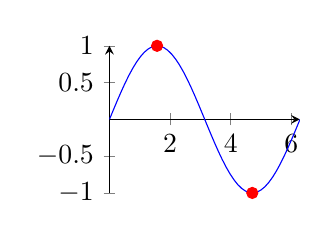
\begin{tikzpicture}
\begin{axis}[width=4cm, xmin=0, xmax=6.28, axis lines=center]
\addplot[blue, samples=50, domain=0:6.28]{sin(deg(x))};
\addplot[red, mark=*]coordinates {(1.57, 1)};
\addplot[red, mark=*]coordinates{(4.71, -1)};
\end{axis}
\end{tikzpicture}

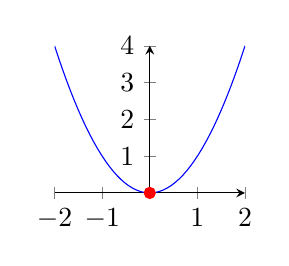
\begin{tikzpicture}
\begin{axis}[width=4cm, xmin=-2, xmax=2, axis lines=center]
\addplot[blue, samples=50, domain=-2:2]{x^2};
\addplot[red, mark=*]coordinates{(0, 0)};
\end{axis}
\end{tikzpicture}

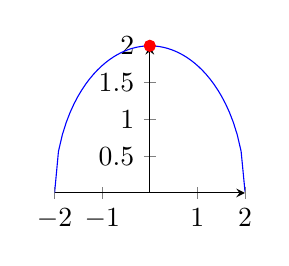
\begin{tikzpicture}
\begin{axis}[width=4cm, xmin=-2, xmax=2, axis lines=center]
\addplot[blue, samples=50, domain=-2:2]{sqrt(4-x^2)};
\addplot[red, mark=*]coordinates{(0, 2)};
\end{axis}
\end{tikzpicture}

You should notice that all of the tangent lines are horizontal. Since the tangent lines at these local extrema have a slope of $0$, that tells us $f'(x)=0$ at these points too. In fact, for \textit{all} local minima and maxima, the value of the derivative is zero at that point. However, the converse statement is not necessarily true: just because the derivative is zero at some $x=c$ it does not mean there is a local extrema at $f(c)$. Consider $f(x) = x^3+3$:

\begin{tikzpicture}
\begin{axis}[axis lines=center]
\addplot[blue, samples=50, domain=-1:1]{x^3+3};
\addplot[red, mark=*]coordinates{(0, 3)};
\addplot[red, samples=50]coordinates{(-0.25, 3) (0.25,3)};
\end{axis}
\end{tikzpicture}

At $x=0$, $f'(x)=0$, but there is not a local extreme. For a local extreme to exist, the graph of $f(x)$ must change from increasing to decreasing, or vice versa. Look at the graph of $x^3+3$ above: the function is increasing for $x<0$ and $x>0$. Another way of saying this is to note that the graph of $f'(x)$ touches but does not cross the x-axis in this case:

\begin{tikzpicture}
\begin{axis}[axis lines = left]
\addplot[blue, samples=50, domain=-2:2]{3*x^2};
\end{axis}
\end{tikzpicture}

If $f(x)$ changes from increasing to decreasing, then $f'(x)$ is changing from positive to negative (i.e. crossing the x-axis). Look at the derivative of $f(x)=\sin{x}$, $f'(x)=\cos{x}$, on the graph below. The x-values where local extrema exist on $f(x)$ are marked in red:

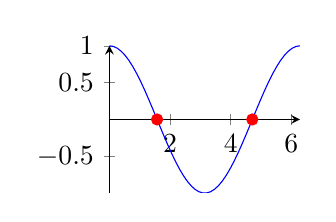
\begin{tikzpicture}
\begin{axis}[width=4cm, xmin=0, xmax=6.28, axis lines=center]
\addplot[blue, samples=50, domain=0:6.28]{cos(deg(x))};
\addplot[red, mark=*]coordinates {(1.57, 0)};
\addplot[red, mark=*]coordinates{(4.71, 0)};
\end{axis}
\end{tikzpicture}

As you can see, local extrema are indicated when $f'(x)$ crosses the x-axis. If $f'(x)$ is negative to the left of $x=c$ and positive to the right, then $f(x)$ has a local minimum at $x=c$. On the other hand, if $f'(x)$ is positive to the left of $x=c$ and negative to the right, then $f(x)$ has a local maximum at $x=c$. 

\subsubsection{Practice}
\begin{Exercise}
    [label=incdec1]
    Let $f$ be the function given by $f(x) = 300x-x^3$. On which of the following intervals is $f$ increasing?
\end{Exercise}
\begin{Answer}
    [ref=incdec1]
    First, we will find $f'$ and set it equal to zero: $$f'(x)=300-3x^2=0$$ $$300=3x^2 \rightarrow x=\pm \sqrt{100} = \pm10$$ (Note: $f'(x) = 3(10-x)(10+x)$, which implies roots at $x=\pm10$. Now we will evaluate the value of $f'(x)$ for $x<-10$, $-10<x<10$, and $x>10$. 
    \begin{center}
        \begin{tabular}{c|c|c|c|c}
        Value of $x$ & (10-x) & (10+x) & $f'(x)$ & $f(x)$ behavior\\
         $x<-10$    &  positive & negative& negative & decreasing\\
         $-10<x<10$    & positive & positive& positive& increasing\\
         $x>10$ & negative & positive & negative & decreasing
        \end{tabular}
    \end{center}
    Therefore, the fucntion is increasing on the interval $x \in [-10, 10]$ because $f'(x) >0$ for $x \in [-10, 10]$.
\end{Answer}

\begin{Exercise}[label=locext1]
Find the intervals on which $f(x)=x^3-3x^2-9x+4$ is increasing or decreasing. Then, find all local minimum and/or maximum values of $f(x)$. 
\end{Exercise}

\begin{Answer}[ref=locext1]
Given $f(x)=x^3-3x^2-9x+4$, it follows that $f'(x)=3x^2-6x-9$. Factoring, we find that $f'(x) = 9(x-3)(x+1)$ and $f'(x) = 0$ when $x=3$ and $x=-1$. We construct our table to help us analyze the value of $f'(x)$ and behavior of $f(x)$ on the whole domain of the function:
\begin{center}
\begin{tabular}{c|c|c|c|c}
	Value of $x$ & $(x-3)$ & $(x+1)$ & $f'(x)$ & $f(x)$ behavior\\
	$x<-1$ & negative & negative & positive & increasing\\
	$-1<x<3$ & negative & positive & negative & decreasing\\
	$x>3$ & positive & positive & positive & increasing
\end{tabular}
\end{center}
So, $f(x)$ is increasing for $x \in (-\infty, -1) \cup (3, \infty)$ and decreasing for $x \in (-1, 3)$. Since $f'(-1)=0$ and changes from positive to negative, $f(x)$ has a local maximum at $x=-1$. And since $f'(3)=0$ and changes from negative to positive, $f(x)$ has a local minimum at $x=3$.
\end{Answer}

\section{Applications in Physics}

In physics, derivatives play a vital role in describing how quantities
change with respect to one another.

\subsection{Velocity and Acceleration}

In kinematics, the derivative of the position function with respect to
time gives the velocity function, and further taking the derivative of
the velocity function gives the acceleration function. For example, if
$s(t)$ represents the position of an object at time $t$, then the
velocity $v(t)$ and acceleration $a(t)$ are given by:

\begin{equation}
v(t) = \frac{ds}{dt} \quad \text{and} \quad a(t) = \frac{dv}{dt} = \frac{d^2s}{dt^2}
\end{equation}

\subsubsection{Practice}

A particle's motion is described by $s(t) = t^3-6t^2+6t$, where $t$ is measured in seconds and $s$ is measured in meters. Answer the following questions about the particle's motion:
\begin{Exercise}[label=velacc1]
Find the velocity at time $t$.
\end{Exercise}

\begin{Answer}[ref=velacc1]
Velocity is the derivative of position. Therefore, $v(t) = s'(t) = 3t^2-12t+6$.
\end{Answer}

\begin{Exercise}[label=velacc2]
What is the velocity after 2s? After 4s?
\end{Exercise}

\begin{Answer}[ref=velacc2]
$$v(2) = 3(2)^2-12(2)+6=-6 \frac{m}{s}$$
$$v(4) = 3(4)^2-12(4)+6=6\frac{m}{s}$$
\end{Answer}

\begin{Exercise}[label=velacc3]
When is the particle at rest?
\end{Exercise}

\begin{Answer}[ref=velacc3]
When the particle is at rest, $v(t) = 0$. 
$$3t^2-12t+6=0$$
$$3(t^2-4t+2)=0$$
$$t^2-4t+2=0$$
This is not easily factorable, so we will use the quadratic formula: $$t=\frac{-(-4)\pm\sqrt{(-4)^2-4(1)(2)}}{2(1)}$$
$$x=\frac{4\pm\sqrt{16-8}}{2}=2\pm\sqrt{2}\approx0.586, 3.414$$
Therefore, the particle is at rest at 0.586s and 3.414s.
\end{Answer}

\subsection{Force and Momentum}

In mechanics, the derivative of the momentum of an object with respect
to time gives the net force acting on the object, as stated by
Newton's second law of motion:

\begin{equation}
F = \frac{dp}{dt}
\end{equation}

where $F$ is the force, $p$ is the momentum, and $t$ is the time.

